\centerline{\bf \Large  РЕШЕНИЯ и КРИТЕРИИ}

\centerline{\bf \Large  9 КЛАСС}


\problem{\textbf{1}} 
Ответ: 2021. Решение. Сумма равна $(10-1)+(100-1)+\ldots+\left(10^{2025}-1\right)=11 \ldots 110-$ $2025=11 \ldots 1109085$, где в числе $11 \ldots 110-2025$ единиц, и, следовательно, в числе $11 \ldots 1109085-2021$ единиц.

\textbf{Критерии.} \\
\textit{6 баллов} $-$ Полностью верное решение, но в конце допущена арифметическая ошибка\\
\textit{3 балла} $-$ Выписано выражение $(10-1)+(100-1)+\ldots+\left(10^{2025}-1\right)$ без дальнейшего решения\\
\textit{0 баллов} $-$  Только ответ\\ 


\problem{\textbf{2}} Пусть за сутки $Y$ клубники съедают насекомые, а $X$ клубники собирает один человек.

Тогда имеем равенство:

$5\cdot(401\cdot X+Y) = 1\cdot(2025\cdot X+Y)$

Из которого получаем: $Y=5X$

Всего клубники растёт в огороде $2030X$

Значит, чтобы собрать за неделю день нужно позвать 284 друга

$7\cdot((284+1)\cdot X+5\cdot X) = 2030X$
\par

\textbf{Критерии.} \\
\textit{0-4 баллов} $-$ Решение пункта А\\
\textit{0-1 балла} $-$ Составление условия пункта Б \\
\textit{0-2 баллов} $-$ Решение пункта Б\\
\textit{0 баллов} $-$ Отсутствие решения пункта А (сразу НОЛЬ! баллов)\\
\textit{0 баллов} $-$ Любой ответ без объяснений\\

\problem{\textbf{3}} Найдём количество чисел, которые делятся на 5: 2025/5=405

Количество чисел, которые делятся на 25: 2025/25=81

Количество чисел, которые делятся на 5, но не делятся на 25: 405-81=324

Которые можем разбить на 162 пары и покрасить каждую в различные цвета.

Каждое число, которое делится на 25, покрасим также в различные цвета.

Максимум можем покрасить в 162+81=243 цвета все числа, чтобы условие задания выполнялось. Следовательно, Очир не может этого сделать.\par

\textbf{Критерии.} \\
\textit{7 баллов} $-$ Полностью верное решение\\
\textit{1 балл} $-$ Найдено количество чисел, которые делятся на 5\\
\textit{1 балл} $-$ Найдено количество чисел, которые делятся на 25\\
\textit{1 балл} $-$ Найдено количество чисел, которые делятся на 5, но не делятся на 25\\ 
\textit{1 балл} $-$ Разбиение 324-ёх чисел на 162 пары и раскрашивание их в 162 различных цвета\\
\textit{1 балл} $-$ Раскрашивание чисел, которые делятся на 25 в 81 различный цвет\\
\textit{0-1 балл} $-$ За все остальные попытки решить задачу\\
\textit{0 баллов} $-$ Любой ответ без объяснений\\


\begin{wrapfigure}{r}{0.1\linewidth}
    \vspace{-7mm}
    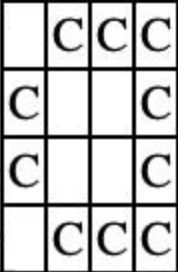
\includegraphics[width=\linewidth]{Секретная информация/УДЕ 2024-2025/Муницип. Решения/slon.png}
\end{wrapfigure}


\problem{4}
Ответ. 10. Решение. Пример с 10 слонами - на рисунке справа. Чтобы доказать, что больше 10 слонов быть не может, покажем, что на полях одного цвета может стоять не больше 5 слонов. Всего есть 8 полей данного цвета. Если слон стоит на угловой клетке, то больше слонов на исходящей из этого угла диагонали нет, то есть всего слонов на клетках этого цвета не больше 5. Если же в угловых клетках слоны не стоят, а во всех 6 оставшихся клетках - стоят, то есть два слона, которых бьют три других, что противоречит условию.

\textbf{Критерии.} \\
\textit{7 баллов} $-$ Полностью верное решение\\
\textit{5 баллов} $-$ Полностью верная оценка\\
\textit{2 балла} $-$ Верный пример (не важно с пояснениями или без)\\
\textit{1 балл} $-$ Сказано, что угловой слон не может бить ни одного другого слона\\
\textit{3 балла} $-$ Доказана оценка только при наличии углового слона\\
\textit{0 баллов} $-$ Решение со словами "рассмотрим наилучший"/"наихудший" случай\\

\problem{5}
Продлим прямую $OV$ до пересечения с $ZD$, допустим, в точке $E$. Исходя из условия $OE$ серединный перпендикуляр к $ZD$. Продлим $ZO$ до пересечения с окружностью $\omega$, допустим, в точке $G$. Тогда $ZG$ --- диаметр окружности $\omega$, а значит продолжение $AM$ попадает в точку $G$. Пусть $\angle ODE = OZE = \alpha$. Тогда из вписанности получаем, что $GAD = \alpha$, а из того что $ABCD$ трапеция получаем, что $AMB = \alpha \ (AD \| BC \text{ АМ секущая}).$ Так как $O$ центр окружности $\omega$, а точка $M$ середина хорды $BC$, то $OM \perp BC$. А значит $\angle OMV = 90 - \alpha$. Стало быть $\angle OMV = \angle EOD = 90 - \alpha$, тогда по теореме об угле между касательной и хордой $OD$ касательная.

\textbf{Критерии.}\\
\textit{7 баллов} $-$ Полностью верное решение\\
\textit{3 балла} $-$ Доказано, что $\angle ZDO = \angle AMB$\\
\textit{1 балл} $-$ Доказано, что $AM$ и $ZO$ пересекаются в одной точке на окружности\\
\textit{1 балл} $-$ Задача решена при определённом расположении точек $A,B,C,D$\\
\textit{0 баллов} $-$ За все остальные попытки решить задачу\\